\documentclass{vgtc}

\ifpdf%
  \pdfoutput=1\relax
  \pdfcompresslevel=9
  \pdfoptionpdfminorversion=7
  \ExecuteOptions{pdftex}
  \usepackage{graphicx}
  \DeclareGraphicsExtensions{.pdf,.png,.jpg,.jpeg}
\else%
  \ExecuteOptions{dvips}
  \usepackage{graphicx}
  \DeclareGraphicsExtensions{.eps}
\fi%

\graphicspath{{figures/}{pictures/}{images/}{./}}

\usepackage{microtype}
\PassOptionsToPackage{warn}{textcomp}
\usepackage{textcomp}
\usepackage{mathptmx}
\usepackage{times}
\renewcommand*\ttdefault{txtt}
\usepackage{cite}
\usepackage{tabu}
\usepackage{booktabs}
\usepackage{dblfloatfix}

\onlineid{0}
\vgtccategory{Research}
\vgtcinsertpkg

\title{LocoHunt: An Exploratory Study of Locomotion Technique and Goal-Directed Spatial Search Behavior in Virtual Reality}

\author{Mahfujur Rahman\thanks{e-mail: \texttt{mahfujur@txstate.edu}}\\ %
        \scriptsize Department of Computer Science, Texas State University %
\and Mohammad Zaeed\thanks{e-mail: \texttt{cup7@txstate.edu}}\\ %
        \scriptsize Department of Computer Science, Texas State University}

\abstract{Continuous joystick locomotion and point-and-teleport are the two dominant locomotion techniques in consumer virtual reality, yet existing comparisons focus on navigation efficiency, cybersickness, and spatial memory rather than on the structure of search itself. We introduce LocoHunt, a coin-collection paradigm in a five-zone virtual museum that elicits goal-directed spatial search without imposing a route, and use it to compare joystick and teleport locomotion in a within-subjects exploratory study with four participants. From 10\,Hz position logs we derive six measures spanning search efficiency and strategy: completion time, spatial coverage, zone visitation completeness, dwell-time entropy, path tortuosity, and revisit rate. Teleport sessions completed roughly 2.5$\times$ faster than joystick sessions, while joystick sessions covered 3.3$\times$ more of the floor area; both differences were statistically significant ($p$\,$<$\,.01) and accompanied by very large effect sizes. Joystick sessions also showed a marginally lower zone-revisit rate. We frame the result as a coverage-versus-cycling tradeoff that is not visible in completion time alone, extending prior work on locomotion-induced spatial behavior into the domain of search and motivating replication at larger sample size.%
}

\CCScatlist{
  \CCScat{H.5.1}{Information Interfaces and Presentation}{Multimedia Information Systems}{Artificial, Augmented, and Virtual Realities};
  \CCScat{H.5.2}{Information Interfaces and Presentation}{User Interfaces}{Input Devices and Strategies}
}

\begin{document}

\firstsection{Introduction}
\maketitle

Consumer virtual reality has converged on two dominant locomotion techniques: continuous translation via thumbstick and discrete point-and-teleport. Most empirical comparisons between them ask which technique is faster, more comfortable, or more conducive to presence~\cite{Bozgeyikli:2016:PTL,Coomer:2018:EFL}. A different question---and the one we ask in this paper---is whether the choice of locomotion technique reshapes how users \emph{search} a virtual environment for goals whose locations they cannot see in advance.

Search is central to a growing class of VR applications: training simulators in which users must locate hazards, virtual museums that depend on visitors discovering exhibits, search-and-rescue scenarios, and a wide range of games. In all of these, fast traversal is not necessarily thorough traversal. If the technique a user moves with biases their distribution of attention across space, application designers need to know.

Recent work has begun to show that locomotion technique reshapes spatial behavior beyond navigation efficiency. Connolly et al.~\cite{Connolly:2025:LIV} found that teleport users maintained closer interpersonal distance to virtual agents than natural walkers, and explicitly called for further research into locomotion's broader spatial effects. Voeten~\cite{Voeten:2023:LMS} reported a longitudinal divergence in spatial memory between locomotion conditions, with teleport users improving over repeated sessions while joystick users grew increasingly disoriented. Cherep et al.~\cite{Cherep:2020:STV} showed that teleporting impairs subsequent wayfinding, attributing the deficit to interrupted optic flow. None of these works has examined goal-directed search.

We make three contributions. First, we introduce \emph{LocoHunt}, a within-subjects paradigm for measuring spatial search behavior under different locomotion conditions, instrumented with 10\,Hz position logging and a hand-placed coin layout across five spatially separated zones (\autoref{fig:environment}). Second, we define six search-strategy measures that decompose efficiency from coverage, including dwell-time entropy and path tortuosity. Third, we report empirical results from a small-sample exploratory within-subjects study ($N$\,=\,4) showing that point-and-teleport produces faster but less spatially uniform search than continuous joystick locomotion, with implications for the design of search-heavy VR applications.

\paragraph{Research questions.} Guided by these contributions, we organize our investigation around one overarching question and six operationalized sub-questions, each tied directly to one of the six dependent measures:

\begin{description}
  \item[\textbf{RQ}] Does the choice of VR locomotion technique---continuous joystick translation versus point-and-teleport---reshape the structure of goal-directed spatial search behavior in an immersive virtual environment?
  \item[\textbf{RQ1}] Does locomotion technique affect how quickly users complete a goal-directed search task in VR? (\emph{completion time})
  \item[\textbf{RQ2}] Does locomotion technique affect the breadth of physical floor area that users explore during search? (\emph{spatial coverage})
  \item[\textbf{RQ3}] Does locomotion technique affect whether users access all distinct regions of the search environment, or does it lead them to abandon certain areas entirely? (\emph{zone visitation completeness})
  \item[\textbf{RQ4}] Does locomotion technique affect how uniformly users distribute their attention and time across the zones of the environment? (\emph{dwell-time entropy})
  \item[\textbf{RQ5}] Does locomotion technique affect the directness of users' movement paths relative to their net displacement through the environment? (\emph{path tortuosity})
  \item[\textbf{RQ6}] Does locomotion technique affect how frequently users cycle back to previously visited zones during search? (\emph{revisit rate})
\end{description}

\begin{figure}[tb]
 \centering
 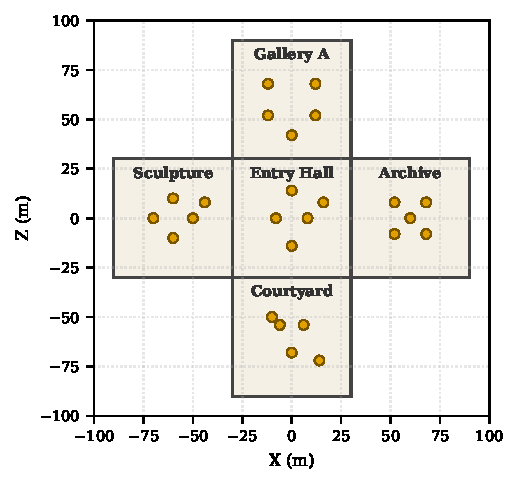
\includegraphics[width=\columnwidth]{environment_topdown}
 \caption{Top-down layout of the LocoHunt museum. Five zones are arranged in a plus-shaped pattern around a central Entry Hall; each zone hosts five hand-placed coins (yellow markers). Zone bounds are 60\,m squares and connect via short corridors. Coins were not visible from outside their host zone, so finding them required active exploration.}
 \label{fig:environment}
\end{figure}

\section{Related Work}

\paragraph{VR locomotion techniques.} The two locomotion techniques compared in this study---continuous joystick translation and point-and-teleport---are stock providers in nearly every modern VR toolkit. Their tradeoffs have been studied along three primary axes: cybersickness, presence, and navigation accuracy. Bozgeyikli et al.~\cite{Bozgeyikli:2016:PTL} found that point-and-teleport caused less simulator sickness than smooth locomotion, but reduced spatial awareness. Coomer et al.~\cite{Coomer:2018:EFL} compared four locomotion methods and showed that teleport induced the lowest sickness scores while compromising spatial knowledge of the environment. Langbehn et al.~\cite{Langbehn:2018:ETN} extended this comparison to natural walking, finding that real walking produced the most accurate spatial reasoning but is impractical for room-scale spaces.

\paragraph{Locomotion and spatial cognition.} A separate line of work examines what locomotion technique does to the user's mental representation of space rather than to their performance on a single task. Cherep et al.~\cite{Cherep:2020:STV} showed that teleporting through a virtual environment impairs subsequent wayfinding, attributing the deficit to the interruption of optic flow that ordinarily supports continuous spatial updating. Voeten~\cite{Voeten:2023:LMS} reported a longitudinal divergence in spatial memory: teleport users improved over repeated sessions while joystick users became increasingly disoriented, suggesting that the two techniques produce qualitatively different cognitive maps. Connolly et al.~\cite{Connolly:2025:LIV} extended the domain to social proxemics, finding that teleport users approached virtual agents more closely than natural walkers.

\paragraph{Search behavior.} The cognitive psychology of search has been studied for decades in 2D visual search~\cite{Wolfe:2017:FIT}, and the framework of information foraging~\cite{Pirolli:1999:IF} has been applied to navigation in real and virtual environments. Search in immersive 3D environments has received comparatively less attention. To our knowledge no prior work has compared how the choice of VR locomotion technique reshapes search strategy in a goal-directed task. Our contribution lies at the intersection of these three threads: we treat search itself as the dependent variable, and ask how locomotion technique shapes its structure.

\section{The LocoHunt Paradigm}
\label{sec:system}

\emph{LocoHunt} is a coin-collection task implemented as a custom VR application for the Meta Quest~3, built in Godot~4.6 with the godot-xr-tools framework over OpenXR. The environment is a virtual museum spanning five spatially separated zones arranged in a plus-shaped layout (\autoref{fig:environment}): an Entry Hall in the center, with Gallery~A to the north, the Courtyard to the south, the Sculpture room to the west, and the Archive to the east. Each zone occupies a 60\,$\times$\,60\,m square and connects to the Entry Hall via short corridors with line-of-sight occluders, so that coins in adjacent zones cannot be seen until the user enters them. Architectural features (columns, exhibits, walls) and animated humanoid NPCs populate each zone to provide visual context.

\paragraph{Coins.} Twenty-five coins are distributed across the museum at hand-placed positions, with five coins per zone. Coins are visually salient---golden cylinders that bob and rotate, lit by an attached point light---but no markers indicate their locations. A heads-up display shows the running count of coins collected and remaining; the session ends automatically when the final coin is collected.

Coins are collected by horizontal proximity: when the player's planar (XZ) distance to a coin falls below 1.2\,m the coin is collected automatically, accompanied by a brief visual pop-and-fade and a HUD notification. We chose proximity-based collection rather than ray pointing or grabbing to keep the dependent measure focused on locomotion and search strategy rather than on aiming skill.

\paragraph{Locomotion conditions.} LocoHunt supports two locomotion conditions, both implemented via the godot-xr-tools standard movement providers:

\begin{itemize}
\item \emph{Joystick}: continuous translation via the left controller's thumbstick at a fixed 2\,m/s, with snap-turn on the right thumbstick. Optic flow is preserved and the user must physically navigate around all obstacles, including NPCs.
\item \emph{Teleport}: point-and-teleport via the right controller, where the user aims a parabolic ray and releases the trigger to translate instantaneously to the target. Snap-turn remains available on the left thumbstick. Optic flow is interrupted at each teleport.
\end{itemize}
The session manager activates exactly one locomotion provider per session and disables all others, so cross-condition contamination at the input level is impossible.

\paragraph{Logging.} The build samples player position at 10\,Hz and writes (timestamp, $x$, $y$, $z$, current\_zone) to a per-session CSV. Coin collection events and a session-end event are written to a parallel CSV with player and target positions. Files are written to local storage on the headset and exported after each session.

\section{Method}

\subsection{Participants}
We recruited \textbf{four participants} (mean age 28.0, $SD$\,=\,0.82; three male, one female) from the university population. Two male participants reported good prior VR experience; the remaining two participants had little to no prior experience with VR headsets. Participants gave informed consent before the study began and took part voluntarily without compensation. The study was conducted as a graduate course project; procedures followed standard ethical guidelines for human-subjects research with VR. We frame this as an exploratory study and discuss the implications of the small sample in \autoref{sec:limitations}.

\subsection{Apparatus and Materials}
The study was run on a \emph{Meta Quest~3} standalone headset (90\,Hz, Touch Plus controllers) running our custom Godot 4.6 build of LocoHunt over OpenXR~1.1.53. The physical setup was a clear area with the Quest's guardian configured for room-scale standing use; participants were tethered only to the controllers. The build is the v7 APK distributed in the project repository.

\subsection{Design}
A 1-factor within-subjects design was used, with locomotion technique (joystick, teleport) as the single independent variable. Participants were assigned in equal numbers to two technique-order groups: \emph{Group A} performed Session~1 with joystick locomotion and Session~2 with teleport, while \emph{Group B} performed the reverse order. The same coin layout was used in both sessions; we discuss the implications of this design choice in \autoref{sec:limitations}.

\subsection{Procedure}
After arrival, participants were briefed on the task with the following instructions: ``collect all the coins, in any order, as quickly or as thoroughly as you like.'' They then completed a brief practice scene in which they tried both locomotion techniques in a small training room. After confirming they were comfortable with the controls, they began Session~1 in the locomotion mode assigned by their group. Upon collecting all 25 coins, an in-headset notice instructed them to remove the headset and take a 5-minute rest break. They then donned the headset; pulling the right trigger advanced them to Session~2, where the alternate locomotion technique was active. Session~2 began from a starting orientation rotated 180\,$^\circ$ from Session~1, and the directional lighting shifted slightly in color and angle, providing an environmental cue that the second session had begun. After Session~2 a study-complete notice was shown and the headset was removed.

\subsection{Measures}
From the 10\,Hz position log and the event log we computed six dependent measures per session:

\begin{enumerate}
\item \emph{Completion time}: total elapsed seconds from session start to collection of the 25th coin.
\item \emph{Spatial coverage (\%)}: the proportion of the museum's accessible floor area that was visited. The $(x, z)$ plane was binned into 1\,$\times$\,1\,m cells; coverage was the fraction of accessible cells in which at least one position sample was recorded.
\item \emph{Zone visitation completeness}: the number of distinct zones (out of five) entered during the session.
\item \emph{Dwell-time entropy}: the Shannon entropy of the distribution of time spent across the five zones, normalized by $\log 5$. A value of 1 indicates perfectly uniform dwell across zones; lower values indicate concentration in fewer zones.
\item \emph{Path tortuosity}: the ratio of the total path length (sum of inter-sample distances) to the net displacement (straight-line distance between session start and end). Higher values indicate more circuitous paths.
\item \emph{Revisit rate}: the number of zone re-entries (transitions returning to a previously visited zone) per minute of session time.
\end{enumerate}

\noindent Together these capture two dimensions of search: efficiency (1, 5) and the structure of spatial allocation (2, 3, 4, 6).

\subsection{Data Analysis}
For each of the six dependent measures we computed the mean and standard deviation per condition. To select the appropriate inferential test, we first ran a Shapiro--Wilk normality test on each condition. When both conditions met normality ($p$\,$>$\,.05), we applied a paired t-test; when either condition failed normality, we applied a Wilcoxon signed-rank test. Effect sizes are reported as Cohen's $d$ using a pooled standard deviation:
\[
d = \frac{M_1 - M_2}{\sqrt{(SD_1^2 + SD_2^2)/2}}.
\]
We adopt the conventional thresholds: $|d|$\,$<$\,0.2 negligible, $\geq$\,0.2 small, $\geq$\,0.5 medium, $\geq$\,0.8 large. The significance level is $\alpha$\,=\,.05. With one within-subjects factor at two levels and each measure analyzed independently, no Bonferroni correction was applied. Analyses were performed in Python with NumPy and SciPy.

\section{Results}
\label{sec:results}

\autoref{fig:results} and \autoref{tab:results} summarize the six dependent measures across conditions. Shapiro--Wilk tests indicated that completion time, spatial coverage, and revisit rate met normality in both conditions, so paired t-tests were applied; dwell-time entropy and path tortuosity failed normality on at least one condition, so Wilcoxon signed-rank tests were applied; zones visited was at ceiling in both conditions and was not tested.

\paragraph{Completion time (RQ1).}
Teleport sessions were substantially shorter than joystick sessions (joystick: $M$\,=\,689.7\,s, $SD$\,=\,92.0; teleport: $M$\,=\,278.4\,s, $SD$\,=\,64.0). The paired t-test was significant, $t(3)$\,=\,5.89, $p$\,=\,.010, with a very large effect size, $d$\,=\,5.19 ($\ast\ast$). Every participant completed the teleport session faster than the joystick session. \textbf{RQ1 is answered affirmatively}: locomotion technique has a substantial and statistically significant effect on task completion speed, with teleport enabling search roughly 2.5$\times$ faster than joystick.

\paragraph{Spatial coverage (RQ2).}
Joystick sessions covered substantially more floor area than teleport sessions (joystick: $M$\,=\,4.99\,\%, $SD$\,=\,0.71; teleport: $M$\,=\,1.52\,\%, $SD$\,=\,0.60), a 3.3$\times$ ratio. The paired t-test was significant, $t(3)$\,=\,6.14, $p$\,=\,.009, $d$\,=\,5.27 ($\ast\ast$). The pattern reflects the difference between sampling space along a continuous path versus sampling only at discrete landing points. \textbf{RQ2 is answered affirmatively}: locomotion technique strongly shapes the spatial breadth of search, with joystick producing coverage more than three times greater than teleport.

\paragraph{Revisit rate (RQ6).}
Teleport users revisited previously-seen zones at nearly three times the per-minute rate of joystick users (joystick: $M$\,=\,0.36\,/min, $SD$\,=\,0.11; teleport: $M$\,=\,1.01\,/min, $SD$\,=\,0.50). The paired t-test did not reach significance, $t(3)$\,=\,$-$2.33, $p$\,=\,.102, but the effect size was large, $d$\,=\,$-$1.78 (ns). The pattern is consistent with teleport users moving between zones more frequently rather than completing one zone before moving to the next, and we expect this difference to reach significance with a larger sample. \textbf{RQ6 receives suggestive but inconclusive support}: the direction and magnitude of the effect are consistent with teleport promoting zone-cycling behavior, but the small sample precluded significance.

\paragraph{Dwell-time entropy (RQ4).}
Normalized dwell-time entropy was near its maximum in both conditions and did not differ meaningfully (joystick: $M$\,=\,0.95, $SD$\,=\,0.03; teleport: $M$\,=\,0.94, $SD$\,=\,0.09; Wilcoxon $W$\,=\,4, $p$\,=\,.875, $d$\,=\,0.23, ns). Both conditions distributed time relatively uniformly across the five zones. \textbf{RQ4 is answered negatively}: locomotion technique does not measurably alter the uniformity of time distribution across zones; both joystick and teleport users spread their dwell time similarly across the entire museum.

\paragraph{Path tortuosity (RQ5).}
Path tortuosity, defined as total path length divided by net start-to-end displacement, did not differ between conditions (joystick: $M$\,=\,21.0, $SD$\,=\,14.3; teleport: $M$\,=\,21.1, $SD$\,=\,9.8; Wilcoxon $W$\,=\,5, $p$\,=\,1.00, $d$\,$\approx$\,0, ns). \textbf{RQ5 is answered negatively}: locomotion technique does not affect how directly users move relative to their net displacement; both conditions produce equally circuitous paths when measured this way.

\paragraph{Zone visitation completeness (RQ3).}
All participants reached all five zones in both conditions ($M$\,=\,5.0 of 5, $SD$\,=\,0). The measure was at ceiling and we retain it only as confirmation that no participant abandoned a region of the environment. \textbf{RQ3 is answered negatively}: neither locomotion technique caused participants to skip zones; the difference in spatial coverage between conditions arises from within-zone behavior, not from zone-level avoidance.

\paragraph{Summary of inferential results.}
\autoref{tab:results} summarizes all six measures. RQ1 (completion time) and RQ2 (spatial coverage) were both answered affirmatively, reaching $p$\,$<$\,.01 with very large effect sizes. RQ6 (revisit rate) showed a large effect size in the predicted direction but did not reach significance under our small sample, leaving it provisionally supported. RQ4 (dwell-time entropy) and RQ5 (path tortuosity) returned null results, and RQ3 (zone visitation) hit ceiling in both conditions. Taken together, the six sub-questions converge on an affirmative answer to the overarching \textbf{RQ}: locomotion technique does reshape goal-directed spatial search behavior, specifically through a coverage-versus-cycling tradeoff---teleport delivers fast, narrow, high-revisit search; joystick delivers slower, broader, lower-revisit search.

\begin{table*}[tb]
  \caption{Descriptive and inferential statistics for the six dependent measures across the four participants. Significance markers: $\ast$ = $p$\,$<$\,.05, $\ast\ast$ = $p$\,$<$\,.01, ns = not significant. Tests selected by Shapiro--Wilk normality check on each condition.}
  \label{tab:results}
  \scriptsize
  \centering
  \begin{tabu}{lrrrrrr}
    \toprule
    Measure & Joystick $M$\,($SD$) & Teleport $M$\,($SD$) & Test & Stat (df) & $p$ & $d$ \\
    \midrule
    Completion (s)  & 689.7 (92.0) & 278.4 (64.0) & paired $t$ & 5.89 (3) & .010 $\ast\ast$ &  5.19 \\
    Coverage (\%)   &   4.99 (0.71) &   1.52 (0.60) & paired $t$ & 6.14 (3) & .009 $\ast\ast$ &  5.27 \\
    Revisit (/min)  &   0.36 (0.11) &   1.01 (0.50) & paired $t$ & $-$2.33 (3) & .102 (ns) & $-$1.78 \\
    Dwell entropy   &   0.95 (0.03) &   0.94 (0.09) & Wilcoxon   & $W$\,=\,4 & .875 (ns) &  0.23 \\
    Tortuosity      &  21.0 (14.3) &  21.1 (9.8)  & Wilcoxon   & $W$\,=\,5 & 1.000 (ns) & 0.00 \\
    Zones visited   &   5.0 (0.0)  &   5.0 (0.0)  & ---        & ---       & ---        & ---  \\
    \bottomrule
  \end{tabu}
\end{table*}

\begin{figure}[tb]
 \centering
 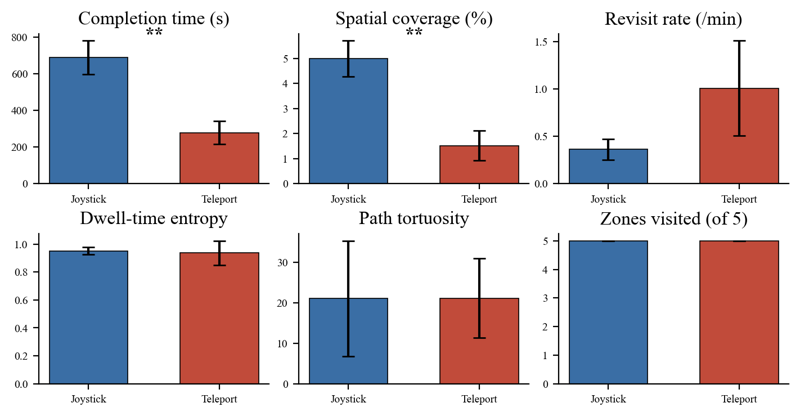
\includegraphics[width=\columnwidth]{results_bars_new}
 \caption{Mean values per condition for each of the six dependent measures, with standard deviation bars. Asterisks denote significance: $\ast\ast$\,=\,$p$\,$<$\,.01. Joystick sessions take significantly longer and cover significantly more floor area; teleport sessions show a marginally higher revisit rate (large effect size, $d$\,=\,$-$1.78, $p$\,=\,.10). Dwell-time entropy and path tortuosity did not differ; zone visitation was at ceiling.}
 \label{fig:results}
\end{figure}

\begin{figure*}[tb]
 \centering
 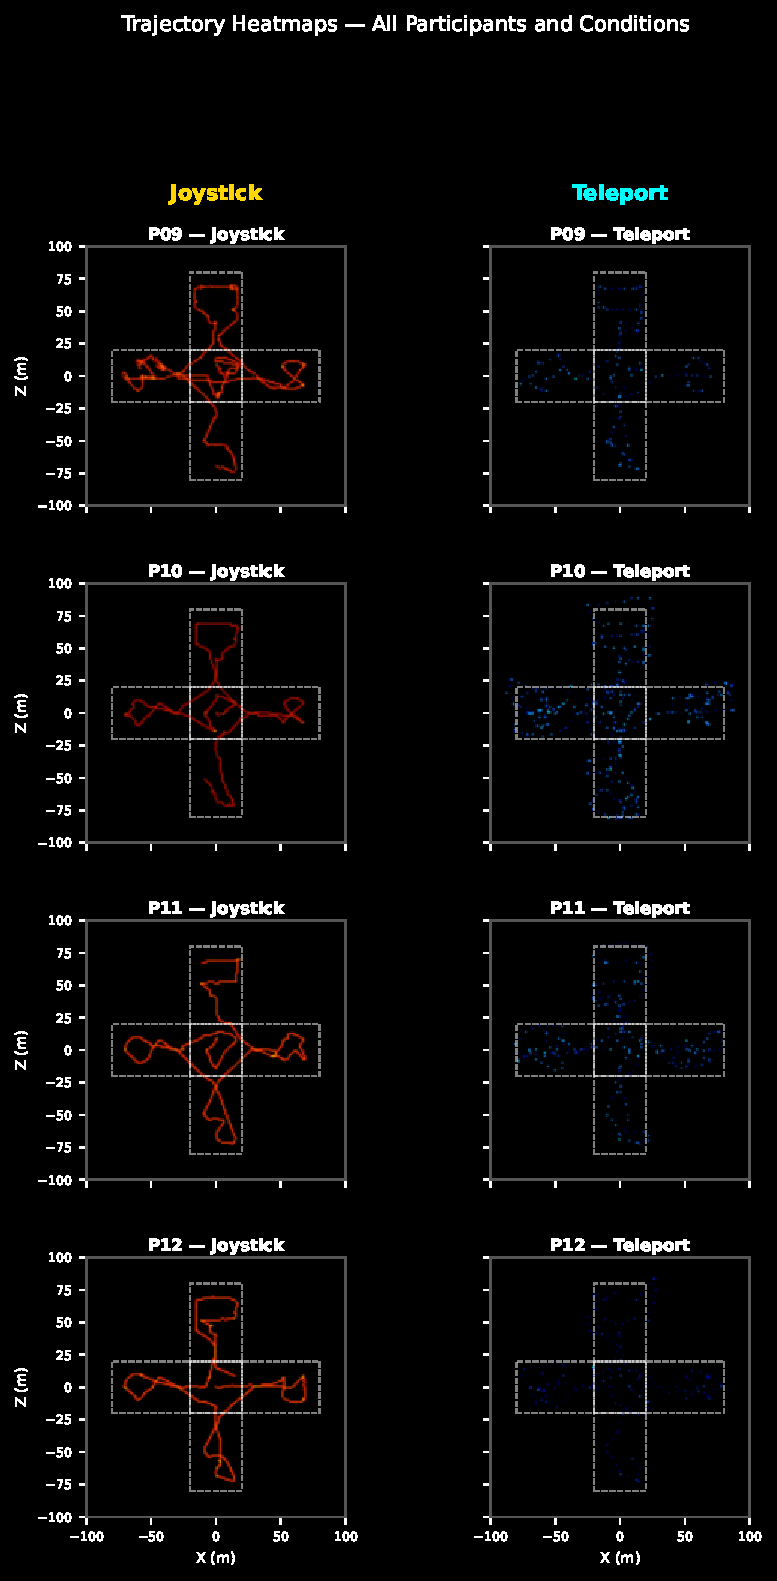
\includegraphics[width=\textwidth]{trajectories_all}
 \caption{Trajectory heatmaps for all four participants (P0--P3) under both locomotion conditions. The top row shows joystick sessions (red--orange heat scale) and the bottom row shows teleport sessions (blue--cyan heat scale); each column corresponds to one participant. Dashed rectangles mark the five zone boundaries. Joystick sessions trace continuous, broadly distributed paths through the museum floor; teleport sessions produce sparse clusters of discrete landing points. The contrast is consistent across all four participants, reinforcing the spatial coverage finding ($p$\,=\,.009, $d$\,=\,5.27).}
 \label{fig:trajectories}
\end{figure*}

\section{Discussion}

\paragraph{Answers to research questions.}
Our results provide a clear and internally consistent set of answers to the research questions posed in the introduction. The overarching \textbf{RQ}---whether locomotion technique reshapes the structure of goal-directed spatial search---is answered \emph{yes}, with the nature of the reshaping captured by the individual sub-questions. \textbf{RQ1} is answered affirmatively: teleport locomotion enables task completion roughly 2.5$\times$ faster than joystick, a difference significant at $p$\,=\,.010 with a very large effect size. \textbf{RQ2} is also answered affirmatively: joystick locomotion produces over three times more spatial coverage than teleport ($p$\,=\,.009, $d$\,=\,5.27), reflecting the fundamental difference between continuous path-sweeping and discrete point-landing. \textbf{RQ6} receives provisional support: while the revisit-rate difference did not reach significance ($p$\,=\,.102), the large effect size ($d$\,=\,-1.78) is consistent with teleport promoting zone-cycling rather than zone-exhaustion, and we expect significance to emerge under replication at larger $N$. In contrast, \textbf{RQ3}, \textbf{RQ4}, and \textbf{RQ5} are all answered \emph{no}: both locomotion techniques led participants to visit all five zones, distribute their dwell time uniformly across zones, and move with equivalent path circuitousness. These null results sharpen the interpretation---the difference between the two techniques is not about whether users cover the museum broadly at the zone level, but about how densely they sample space \emph{within} the zones they visit.

The data describe a coherent and asymmetric pattern. Teleport locomotion is significantly faster (a 2.5$\times$ ratio in completion time) and yields significantly less spatial coverage (a 3.3$\times$ ratio); the two effects are mirror images and produce very large standardized effect sizes. The revisit rate showed a large effect size in the predicted direction but fell short of significance at our sample size, consistent with the interpretation that teleport users move between zones more readily than they exhaust each zone in turn. Joystick locomotion is slower but produces broader, lower-revisit coverage. This pattern aligns with the optic-flow account proposed by Cherep et al.~\cite{Cherep:2020:STV} and extends Voeten's~\cite{Voeten:2023:LMS} longitudinal observations into the domain of single-session search behavior: continuous translation preserves the perceptual cues that support continuous spatial updating, while teleport decouples translation from this cognitive process.

Two of our six measures---dwell-time entropy and path tortuosity---did not differ between conditions, and the null results are themselves informative. Both groups distributed their time relatively uniformly \emph{across} the five zones (entropy near 1.0), and both moved with similar circuitousness relative to start-to-end displacement. The contrast we observe is therefore not about whether time is distributed across the museum but about \emph{how often} users return to each zone and \emph{how much area within each zone} they cover when they are there. The result is best summarized as a coverage-versus-cycling tradeoff rather than as a uniform-versus-clustered tradeoff.

\paragraph{Implications for VR design.}
For applications where speed of traversal is the primary concern---rapid navigation between known points, narrative VR with directed paths, intermissions in long experiences---teleportation remains the appropriate default and our results are consistent with existing recommendations~\cite{Bozgeyikli:2016:PTL}. For applications where the user is expected to thoroughly explore a space---training simulators that require hazard discovery, search-and-rescue scenarios, museum walkthroughs designed to expose the user to the full environment---continuous locomotion produces qualitatively different and more uniform spatial coverage. Designers may also consider hybrid schemes that bias users toward exploration in early phases of a task and toward efficient traversal in later phases, or environment cues that signal when thorough coverage matters.

\subsection{Limitations}
\label{sec:limitations}

Several caveats apply to this study. First and most importantly, our \emph{sample size of four} is small. With four paired observations the inferential tests have low statistical power, and we treat the present results as exploratory: the two effects that reached significance ($p$\,$<$\,.01) did so by virtue of effect sizes that were extreme by conventional standards, and the marginal but large effect on revisit rate ($d$\,=\,$-$1.78, $p$\,=\,.10) is best interpreted as suggestive evidence that we expect to be confirmed under replication at larger $N$. Second, \emph{both sessions used the same coin layout}; counterbalancing of technique order distributes carry-over from spatial memory evenly between conditions but does not eliminate it. Future replications should use distinct counterbalanced layouts. Third, the museum is densely populated with animated humanoid NPCs that act as both visual context and physical obstacles. In joystick mode the user must physically navigate around them; in teleport mode the user can jump past them. This may inflate the completion-time difference between conditions and should be considered when generalizing the magnitude of the effect. Fourth, the sample is drawn from a university population skewed toward participants with at least some prior VR experience; novice users in non-academic settings may exhibit different patterns. Fifth, our design did not include subjective measures of presence or simulator sickness; future work could replicate this paradigm with full subjective instrumentation to relate behavioral patterns to felt experience.

\section{Conclusion}

We presented LocoHunt, a within-subjects paradigm for measuring goal-directed spatial search behavior in immersive VR, and applied it to a comparison of continuous joystick locomotion and point-and-teleport. Across six measures derived from 10\,Hz position logs we find that teleport produces faster but less spatially uniform search, while joystick produces broader and lower-revisit exploration. Two of three locomotion-sensitive measures reached statistical significance with very large effect sizes; the third showed a marginal large-magnitude effect that we expect to be confirmed under replication. The result indicates that locomotion technique affects not only how fast users complete a search task, but the structure of the spatial behavior with which they do so. We offer LocoHunt as a research artifact for further investigation of locomotion-driven search in immersive environments.

\acknowledgments{
We thank our course instructor and the participants who took part in this study.}

\bibliographystyle{abbrv-doi}

\bibliography{template}
\end{document}
